\documentclass[a4paper,12pt]{article}
\usepackage[utf8]{inputenc}
\usepackage[T2A]{fontenc}
\usepackage[russian]{babel}
\usepackage{amsmath, amssymb, amsfonts, amsthm}
\usepackage{graphicx}
\usepackage{geometry}
\usepackage{float}
\usepackage[hidelinks, pdfencoding=auto, psdextra]{hyperref}
\usepackage{tocloft}
\usepackage{fancyhdr}
\usepackage{enumitem}
\usepackage{listings}
\usepackage{xcolor}
\usepackage{subcaption}

\geometry{top=2cm, bottom=2cm, left=2cm, right=2cm}
\setlength{\headheight}{14.5pt}

\begin{document}

\begin{titlepage}
    \centering
    {\Large \bfseries Федеральное государственное автономное образовательное учреждение высшего образования «Национальный исследовательский университет ИТМО» \par}
    
    {\large Факультет программной инженерии и компьютерной техники \par}
    \vspace{2cm}
    {\LARGE Домашнее задание №6 \par}
    \vspace{0.5cm}
    \vspace{2cm}
    \vfill
    \begin{flushright}
        \large
        \textbf{Выполнил:} \\
        Шулай Роман \\
        Группа P3115 \\
        \vspace{1cm}
        \textbf{Преподаватель:} \\
        Поляков Владимир Иванович \\
    \end{flushright}
    \vfill
    {\large Санкт-Петербург \\ 2026 год}
\end{titlepage}
\newpage
\setcounter{page}{2}

\noindent
Построим знаковый ориентированный граф в области взаимодействия технологических корпораций и их IT-продуктов. Ребро $(e_i,e_j)$ будет означать, что $e_i$ и $e_j$ взаимосвязаны. Если на ребре стоит $+$, то связь между ними положительная. Если на ребре стоит $-$, то отрицательная.

\begin{figure}[H]
    \centering
    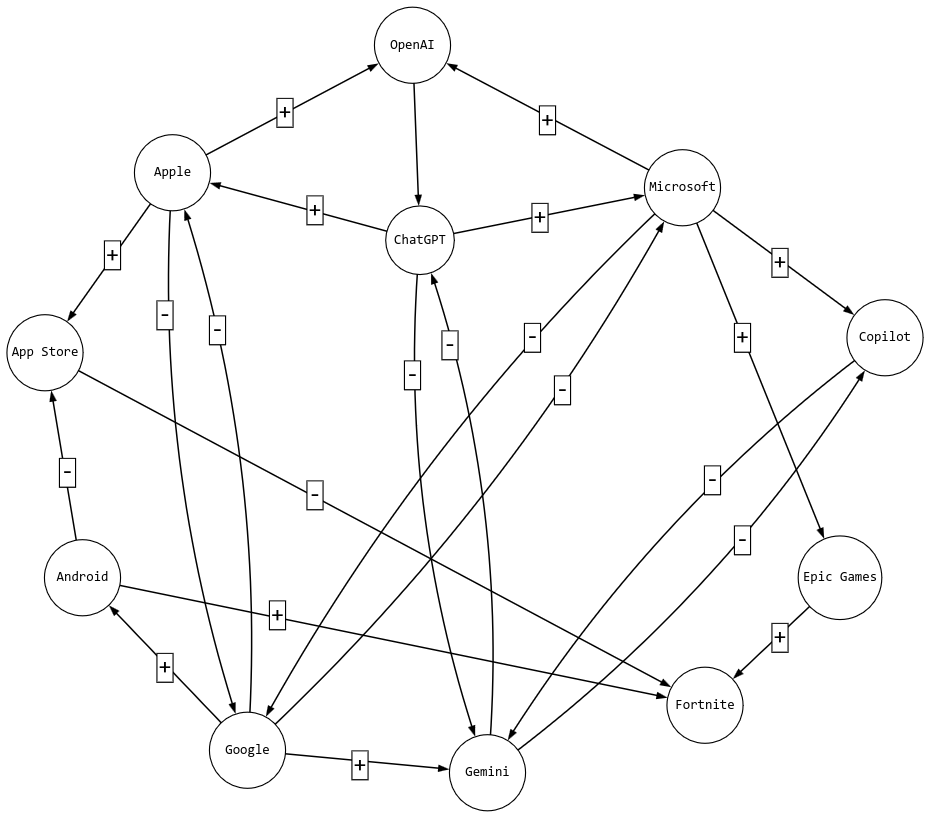
\includegraphics[width=1.1\linewidth]{images/6/graph.png}
\end{figure}

\end{document}